\documentclass{amsart}

%\documentclass[10 pt]{amsart}

\usepackage[ocgcolorlinks,linktoc=all]{hyperref}
\hypersetup{citecolor=blue,linkcolor=red}
\usepackage[parfill]{parskip}
\usepackage{graphicx}

%\usepackage{amsthm}
\usepackage{cleveref}
\crefname{lemma}{Lemma}{Lemmata}
\crefname{equation}{equation}{equations}

\newtheorem{theorem}{Theorem}
\newtheorem{lemma}[theorem]{Lemma}
\newtheorem{proposition}[theorem]{Proposition}
\newtheorem{corollary}[theorem]{Corollary}

\newtheorem*{thmA}{Theorem}
\newtheorem*{thmB}{Theorem}
\newtheorem*{rem}{Remark}
\newtheorem*{thmmain}{Theorem}
\newtheorem*{propmain}{Proposition}

\theoremstyle{definition}
\newtheorem{definition}[theorem]{Definition}
\newtheorem{example}[theorem]{Example}
\newtheorem{xca}[theorem]{Exercise}

\theoremstyle{remark}
\newtheorem{remark}[theorem]{Remark}

\numberwithin{equation}{section}

%Symbols
\renewcommand{\~}{\tilde}
\renewcommand{\-}{\bar}
\newcommand{\bs}{\backslash}
\newcommand{\cn}{\colon}
\newcommand{\sub}{\subset}

\newcommand{\N}{\mathbb{N}}
\newcommand{\R}{\mathbb{R}}
\newcommand{\Z}{\mathbb{Z}}
\renewcommand{\S}{\mathbb{S}}
\renewcommand{\H}{\mathbb{H}}
\newcommand{\C}{\mathbb{C}}
\newcommand{\K}{\mathbb{K}}
\newcommand{\Di}{\mathbb{D}}
\newcommand{\B}{\mathbb{B}}
\newcommand{\8}{\infty}

%Greek letters
\renewcommand{\a}{\alpha}
\renewcommand{\b}{\beta}
\newcommand{\g}{\gamma}
\renewcommand{\d}{\delta}
\newcommand{\e}{\epsilon}
\renewcommand{\k}{\kappa}
\renewcommand{\l}{\lambda}
\renewcommand{\o}{\omega}
\renewcommand{\t}{\theta}
\newcommand{\s}{\sigma}
\newcommand{\p}{\varphi}
\newcommand{\z}{\zeta}
\newcommand{\vt}{\vartheta}
\renewcommand{\O}{\Omega}
\newcommand{\D}{\Delta}
\newcommand{\G}{\Gamma}
\newcommand{\T}{\Theta}
\renewcommand{\L}{\Lambda}

%Mathematical operators
\newcommand{\INT}{\int_{\O}}
\newcommand{\DINT}{\int_{\d\O}}
\newcommand{\Int}{\int_{-\infty}^{\infty}}
\newcommand{\del}{\partial}

\newcommand{\inpr}[2]{\left\langle #1,#2 \right\rangle}
\newcommand{\fr}[2]{\frac{#1}{#2}}
\newcommand{\x}{\times}

\DeclareMathOperator{\dive}{div}
\DeclareMathOperator{\id}{id}
\DeclareMathOperator{\pr}{pr}
\DeclareMathOperator{\Diff}{Diff}
\DeclareMathOperator{\supp}{supp}
\DeclareMathOperator{\graph}{graph}
\DeclareMathOperator{\osc}{osc}
\DeclareMathOperator{\const}{const}
\DeclareMathOperator{\dist}{dist}
\DeclareMathOperator{\loc}{loc}

%Environments
\newcommand{\Theo}[3]{\begin{#1}\label{#2} #3 \end{#1}}
\newcommand{\pf}[1]{\begin{proof} #1 \end{proof}}
\newcommand{\eq}[1]{\begin{equation}\begin{alignedat}{2} #1 \end{alignedat}\end{equation}}
\newcommand{\IntEq}[4]{#1&#2#3	 &\quad &\text{in}~#4,}
\newcommand{\BEq}[4]{#1&#2#3	 &\quad &\text{on}~#4}
\newcommand{\br}[1]{\left(#1\right)}



%Logical symbols
\newcommand{\Ra}{\Rightarrow}
\newcommand{\ra}{\rightarrow}
\newcommand{\hra}{\hookrightarrow}
\newcommand{\mt}{\mapsto}

% Aleksandrov Reflection Macros
\DeclareMathOperator{\reflectionvector}{V}
\DeclareMathOperator{\reflectionangle}{\delta}
\newcommand{\reflectionplane}[1][\reflectionvector]{\ensuremath{P_{#1}}}
\newcommand{\reflectionmap}[1][\reflectionvector]{\ensuremath{R_{#1}}}
\newcommand{\reflectionset}[2][\reflectionvector]{\ensuremath{{#2}_{#1}}}
\newcommand{\reflectionhalfspace}[1][\reflectionvector]{\ensuremath{\reflectionset[{#1}]{H}}}
\DeclareMathOperator{\vertvec}{e}
\DeclareMathOperator{\origin}{O}
\DeclareMathOperator{\radialprojection}{\pi}
\DeclareMathOperator{\height}{h}
\DeclareMathOperator{\equator}{E}
\newcommand{\ip}[2]{\ensuremath{\langle{#1},{#2}\rangle}}
\DeclareMathOperator{\intersect}{\cap}
\DeclareMathOperator{\union}{\cup}
\DeclareMathOperator{\nor}{\nu}
\DeclareMathOperator{\basepoint}{p_0}
\DeclareMathOperator{\radialdistance}{r}

%Fonts
\newcommand{\mc}{\mathcal}
\renewcommand{\it}{\textit}
\newcommand{\mrm}{\mathrm}

%Spacing
\newcommand{\hp}{\hphantom}


\parindent 0 pt

\protected\def\ignorethis#1\endignorethis{}
\let\endignorethis\relax
\def\TOCstop{\addtocontents{toc}{\ignorethis}}
\def\TOCstart{\addtocontents{toc}{\endignorethis}}

%\usepackage[left=1in,right=1in,top=1in,bottom=1in]{geometry}
\begin{document}

\title[Ancient solutions to curvature flows in the sphere]
 {On the classification of ancient solutions to curvature flows on the sphere}

\curraddr{}
\email{}
\date{\today}

\dedicatory{}
\subjclass[2010]{}
\keywords{}

\begin{abstract}
We consider the evolution of hypersurfaces on the unit sphere $\mathbb{S}^{n+1}$ by 1-homogeneous, convex functions of principal curvatures. Our main result states that the only convex, ancient solutions of shrinking curvature flows with 1-homogeneous, convex speeds are shrinking geodesic spheres. The main tools are  differential Harnack inequalities, a rigidity result in the sphere, and an Aleksandrov reflection argument. We also obtain Harnack inequalities for flows by $\a$-power of the mean curvature with $0<\alpha<1$. We introduce the notion of `quasi-ancient` solutions, which play a similar role to ancient solutions for flows that do not admit non-trivial ancient solutions. The techniques presented here in fact allow us to prove that any convex, quasi-ancient solution of a curvature flow which satisfies a uniform bound on the second fundamental form backwards in time must be a family of shrinking geodesic spheres. As an example we treat quasi-ancient solutions of $H^{\a}$-flow with $0<\a<1$.
\end{abstract}

\maketitle

\section{Introduction}

We consider the evolution of a hypersurface $M^n$ by
\eq{\label{eq:CurvFlow}
\partial_tx=-\varphi(f)\nu,~ x:M^n\times[0,T)\to M_K,
}
where \(M_K\) is the simply connected space form of constant sectional curvature \(K\), and $f\in C^{\8}(\G_+)$ is a strictly monotone, 1-homogeneous, symmetric function on the eigenvalues of Weingarten map \(\mathcal{W}\) (principal curvatures) \(\kappa_1, \cdots, \kappa_n\).

\section{Preliminaries}

We will need some notation for derivatives of the speed \(\varphi\). Let us write
\[
\varphi^{i}_{j} = \frac{\partial \varphi}{\partial h^{j}_{i}}
\]
for the first partial derivatives of \(\varphi\). As a function of the metric and second fundamental form,
\[
\varphi(g, h) = \varphi(g^{ik} h_{kj}),
\]
we write
\[
\varphi^{ij} = \frac{\partial\varphi}{\partial h_{ij}}, \quad \varphi^{ij,kl} = \fr{\partial^2\varphi}{\partial h_{kl} \partial h_{ij}}.
\]

Let us also define the operator
\[
\Box = \varphi^{ij} \nabla^2_{ij}
\]

\subsection{Evolution equations}
\eq{
 \label{eq:delt_weingarten_box} 
\partial_t h_i^j &= \Box h_i^j + \varphi^{kl} (h^2)_{kl} h_i^j - (\varphi^{kl}h_{kl} - \varphi) (h^2)_i^j + \varphi^{kl,rs}\nabla_i h_{kl}\nabla^j h_{rs} \\
& \quad + K \{(\varphi + \varphi^{kl}h_{kl}) \delta_i^j - \p^{kl}g_{kl} h_i^j\}
}

\eq{\label{eq:delt_speed} \partial_t \varphi = \Box \varphi + \varphi\varphi^{ij}(h^2)_{ij} + K \varphi\varphi^{ij}g_{ij}}


\section{Ancient and quasi-ancient Solutions}

\subsection{Backwards Limit}
We consider the spherical ambient space, $K=1,$ without further mention, and we are interested in solutions with maximal possible lifetime. To understand this maximal time, we define $T_S$ to be the lifespan of \it{the} convex spherical solution of \eqref{eq:CurvFlow}. By the convex spherical solution we mean a family of geodesic spheres shrinking under the flow \eqref{eq:CurvFlow} collapsing to a point at time $t=0$ and existing on the maximal interval \((-T_S, 0)\). For 1-homogeneous $\p$, \(T_S = \infty\), but for $\alpha$-homogeneous $\p$ with $\alpha<1$, \(T_S\) is finite.

\begin{lemma}
 Consider \eqref{eq:CurvFlow} with speed \(\p = H^{\alpha}\) for \(\alpha \in (0,1)\). Then a flow of strictly convex geodesic spheres has a finite lifespan, i.e., let $S_r(p)$ be a geodesic sphere in $\S^{n+1}$ around $p\in \S^{n+1}$. Then the flow exists only for a finite time interval \((-T_S,0)\) with \(0 < T_S < \infty\), collapsing to a point at \(t=0\) and converging to an equator at \(t=T_S\).
\end{lemma}

\begin{proof}
Since $H$ is constant on a geodesic sphere, for a spherical flow the evolution equation for $\p=H^{\a}$ yields
\eq{\fr{d}{dt}H^{\a}\geq \a n H^{2\a-1}.}
This yields
\eq{\fr{d}{dt}H\geq nH^{\a}.}
Since the right hand side remains strictly positive under this ODE we obtain finite lifespan forward in time.
Convexity and integration over some interval $(a,b)$ yield
\eq{0\leq H^{1-\a}(a)\leq H^{1-\a}(b)-(1-\a)n(b-a).}
Letting $a\ra-\8$ gives finite existence backwards in time.
\end{proof}

\begin{lemma}
Let $x$ be a convex solution of \eqref{eq:CurvFlow}, defined on the open interval $(-T,0),$ where $0$ is the collapsing time, then $T\leq T_S.$
\end{lemma}

\begin{proof}
Suppose $T>T_S+\e$ for some $\e>0$. Since $M=M_{-T_S-\fr{\e}{2}}$ bounds a convex body $\hat{M}$, it strictly contained in an open hemisphere due to the classical paper \cite{CarmoWarner:/1970}. Then there exists a geodesic sphere $S$ with $\hat{M}\sub\hat{S}.$ By the avoidance principle the flow with initial hypersurface $M$ collapses before the spherical flow contradicting $T>T_S$.
\end{proof}

Due to this lemma the following definition is reasonable.

\begin{definition}
A convex solution of \eqref{eq:CurvFlow} defined on an interval $(-T,0)$ is called \it{quasi-ancient}, if $T=T_S$.
\end{definition}
The term ancient is reserved for the situation when \(T_S=\infty\), and by the definition, ancient solutions are also quasi-ancient.

The aim of this section is to prove that for a quasi-ancient solution of \eqref{eq:CurvFlow} the backwards limit of the flow hypersurfaces \it{with bounded mean curvature}, $M_t$ is an equator for $t\ra -T_S$. We will use the method of \cite{MakowskiScheuer:/2013} to achieve this.
For 1-homogeneous, convex speeds, Proposition \ref{cor:boundedH} gives a bound on mean curvature for ancient solutions. For quasi-ancient solutions, the Harnack inequality does not in general give such a bound, since we cannot send \(t \to -\infty\) whenever \(T_S\) is finite. One can envisage backwards limits as convex polyhedra and hence with unbounded \(H\), but it is not clear that these can arise as backwards limits of quasi-ancient solutions. Thus at this stage we must make the additional assumption that \(H\) is bounded for quasi-ancient solutions.

\begin{proposition}
Let $f$ be a strictly monotone, $1$-homogeneous curvature function and let either $f$ be concave and 
\eq{\fr{H}{f}\leq c,}
or let $f$ be convex. Then any strictly convex ancient solution of the flow \eqref{eq:CurvFlow} with speed $\p(f)=f$ is a contraction of geodesic spheres.
\end{proposition}

\pf{
There are various approaches. Let us use the standard maximum principle approach if $f$ is concave. For inverse concave $f$ we use a recent non-collapsing result, cf.~\cite{AndrewsLangford:01/2014}. So let us assume that $f$ is concave. The tensor
\eq{w^j_i=\fr{h^j_i}{f}}
satisfies the evolution equation
\eq{\del_tw^j_i&=\Box w^j_i-2Kf^{kl}g_{kl}w^j_i+2K\d^j_i\\
			&\hp{=}+f^{kl,rs}\nabla_ih_{kl}\nabla^jh_{rs}+2f^{kl}\nabla_kh^j_i\nabla_l\br{\fr{1}{f}}.}
Hence, due to the concavity of $f$ we have for fixed index $i:$
\eq{\del_t\br{w^i_i-\fr{1}{n}}&\leq\Box\br{w^i_i-\fr{1}{n}}-2nK\br{w^i_i-\fr{1}{n}}+2f^{kl}\nabla_kh^i_i\nabla_l\br{\fr{1}{f}}}
At a spatial maximum of $w^i_i-\tfrac{1}{n}$ we have
\eq{0=\nabla_k \br{\fr{h^i_i}{f}}=\fr{\nabla_k h^i_i}{f}+h^i_i\nabla_k\br{\fr{1}{f}}}
and hence by the maximum principle we obtain the bound
\eq{w^i_i-\fr 1n\leq c_0e^{-2nKt},}
where $c_0$ is the upper bound for the function on the left-hand side at $t=0.$
Starting the flow at an arbitrary $s<0$ we find
\eq{\fr{\k_n}{f}\leq \fr 1n+c_se^{-2nK(t-s)}.}
If $K=1,$ letting $s\ra-\8,$ we obtain at every time $t<0$ that 
\eq{\k_n\leq \fr{f}{n}.}
This is only possible for totally umbilical hypersurfaces.
            
}

\begin{proposition}
\label{cor:boundedH}
Suppose $f$ is a convex curvature function. Then any convex ancient solution of the contracting flow with speed $\p(f)=f$ satisfies
\[\partial_t \p-b^{ij}\nabla_i\p\nabla_j\p\geq 0.\]
In particular, for all $t\le -1$ we have
$H(\cdot,t)\leq c.$
Here $c<\infty$ depends only on $M_{-1}.$
\end{proposition}
\begin{proof}
For any $t>s$, the  Harnack estimate of Theorem \ref{thm:main A} implies that
$$\partial_t \p-b^{ij}\nabla_i\p\nabla_j\p+\frac{n}{2}\frac{\p}{t-s}>0.$$
Allowing $s\to-\infty$ proves the first claim. For the second claim, observe that for any 1-homogeneous convex $f$ we have \[f\ge \frac{f(1,\cdots,1)}{n}H,\]
see \cite[Chapter 2]{Gerhardt:/2006}. Therefore, ancient solutions satisfy
\[H(\cdot,t)\leq \frac{n}{f(1,\cdots,1)}\p(\cdot,t)\leq \frac{n}{f(1,\cdots,1)}\p(\cdot,0). \]
\end{proof}

\begin{lemma}\label{ISC}
Let $x$ be a quasi-ancient solution of \eqref{eq:CurvFlow}. Then there holds:\\

(i)~For all $t_0<0$ there exists a uniform radius $R>0,$ such that the enclosed convex bodies $\hat{M}_t,$ $-T_S<t\leq t_0,$ of the flow hypersurfaces $M_t$ satisfy a uniform interior sphere condition with radius $R.$\\

(ii)~For every $y_0\in\mrm{int}~\hat{M}_{t_0}$ the hypersurfaces $M_t,$ $-T_S<t\leq t_0$ can be written as a graph in geodesic polar coordinates around $y_0$ and the corresponding graph functions satisfy uniform $C^2$-estimates.
\end{lemma}

\pf{
Fix an interior point $y_0\in \mrm{int}~\hat{M}_{t_0}.$ Since for a contracting flow the enclosed convex bodies of the flow hypersurfaces are strictly decreasing, they are strictly increasing backwards in time. By \cite[Lemma~3.9]{MakowskiScheuer:/2013} there exists a closed hemisphere $\mc{H}(x_0),$ such that
\eq{\hat{M}_t\sub\mc{H}(x_0).}
In our situation all hypersurfaces $M_t,$ $-T_S<t\leq t_0,$ satisfy
\eq{B_{\e}(y_0)\sub \mrm{int}~\hat{M}_t}
and
\eq{B_{\e}(\hat{y}_0)\sub \hat{M}_t^c}
with a uniform $\e,$ where $\hat{y}_0$ denotes the antipodal point of $y_0.$
Now we prove the two claims.\\

(i)~Consider the stereographic projection with $\hat{y}_0$ corresponding to infinity. The image hypersurfaces are then strictly convex hypersurfaces in Euclidean space with uniformly bounded second fundamental form. Blaschke's rolling theorem, cf.~\cite{Blaschke:/1956}, gives the interior sphere condition.\\

(ii)~
Write the $M_t$ as graphs in geodesic polar coordinates around $y_0,$
\eq{M_t=\{(r,x^i)\cn r=u(t,x^i)\},}
where $r$ describes the geodesic distance to $y_0.$ In these coordinates the spherical metric takes the form
\eq{d\-s^2=dr^2+\sin^{2}r\s_{ij}dx^idx^j,}
where $(\s_{ij})$ is the round metric of $\S^n.$

Hence on the set in which the $M_t$ range, the metrics $\-g_{ij}=\sin^2r\s_{ij}$ and $\s_{ij}$ are equivalent.
Due to \cite[Thm.~2.7.10]{Gerhardt:/2006} for all convex hypersurfaces $M_t$ the quantity
\eq{v^2=1+\-g^{ij}\nabla_iu\nabla_ju}
is uniformly bounded by a constant which only depends on $\e.$
Hence by the equivalence of norms the $M_t$ are uniformly $C^1$-bounded in the sense that the corresponding functions $u(t,\cdot)$ are uniformly $C^1(\S^n)$-bounded.
A straightforward computation yields the following representation of the Weingarten map in terms of the function $u,$ namely
\eq{h^i_j=\fr{\vt'}{v\vt}\d^i_j+\fr{\vt'}{v^3\vt^3}\nabla^iu\nabla_ju-\fr{\~g^{ik}}{v\vt^2}\nabla^2_{kj}u,}
where $\~g^{ij}$ is the inverse of $\~g_{ij}=\vt^{-2}g_{ij},$ $\vt(r)=\sin r$ and covariant derivatives as well as index raising is performed with respect to $\s_{ij},$ compare for example \cite[(3.82)]{Scheuer:05/2015}. Due to the curvature estimates we obtain uniform $C^2(\S^n)$-estimates.
}

\begin{corollary}\label{Backlimit}
Let $x$ be a quasi-ancient solution of \eqref{eq:CurvFlow}. Then there exists a unique backwards limiting hypersurface $M_{-T_S}$ and the flow hypersurfaces $M_t$ converge to $M_{-T_S}$ in $C^{1,\b},$ $0<\b<1,$ in the sense that for a common graph representation as in Lemma \ref{ISC} there holds
\eq{u(t,\cdot)\ra u(-T_S,\cdot)}
in the norm of $C^{1,\b}(\S^n).$
\end{corollary}

\pf{
Due to the pointwise monotonicity of $u(t,\cdot)$ backwards in time we obtain a pointwise limit. The $C^{1,\b}$-convergence follows from compactness.
}

\begin{theorem}
\label{thm:backwardslimit}
The hypersurface $M_{-T_S}$, defined in Corollary \ref{Backlimit}, is an equator.
\end{theorem}

\pf{
Since the convex bodies $\hat{M_t}$ are increasing backwards in time and due to the uniform convergence of $M_t$ to $M_{-T_S},$ the set
\eq{\hat{M}_{-T_S}:=\overline{\bigcup_{t<0}\hat{M}_t}}
is a compact body with
\eq{\del \hat{M}_{-T_S}=M_{-T_S}.}
Since $\mrm{int}(\hat{M}_{-T_S})$ is a strictly convex set, it is especially weakly convex in a hemisphere in the sense of \cite[Def.~3.2]{MakowskiScheuer:/2013}. Thus $\hat{M}_{-T_S}$ is a weakly convex body in a hemisphere. The proof of \cite[Lemma~6.1]{MakowskiScheuer:/2013} can literally be applied to show that $\hat{M}_{-T_S}$ satisfies a uniform interior sphere condition as well.
We can apply \cite[Thm.~1.1]{MakowskiScheuer:/2013} and obtain that $\hat{M}_{-T_S}$ is either strictly contained in an open hemisphere or is equal to a closed hemisphere. The first alternative is not possible since the solution is quasi-ancient. We conclude that $\del \hat{M}_{-T_S}=M_{-T_S}$ is an equator of $\S^{n+1}.$
}


\subsection{Aleksandrov Reflection}

In this section, we use Theorem \ref{thm:backwardslimit} to classify convex, embedded, (quasi-)ancient solutions of contracting curvature flows on \(\S^{n+1}\) as either equators or shrinking geodesic spheres. The proof uses Aleksandrov reflection as in \cite{bryanlouie,2015arXiv150802821B}. Here we give a very general version with minimal assumptions on the flow: all we require is that the flow limits to an equator at $-T_S$ and that the maximum principle holds forward in time.

We begin with some preliminaries of the Aleksandrov reflection on \(\S^{n+1}\). First, we will work relative to the limiting equator obtained in Theorem \ref{thm:backwardslimit}, denoted by $\equator = M_{-T_S}$. The equator \(\equator\) determines two \emph{open} hemispheres \(H^{\pm}\) with centers \(\pm \basepoint\) and we assume the flow is contained in the upper hemisphere, $M_t \subset H^+$. It's convenient to make use of the ambient Euclidean space, \(\R^{n+2}\) with \(\S^{n+1} \subset \R^{n+2}\) via the standard embedding. Let \(\vertvec = \overrightarrow{\origin\basepoint}\) be the unit vector in \(\R^{n+2}\) that points from the origin \(\origin\) to \(\basepoint\); the ``vertical direction''. 

To define the Aleksandrov reflection, let \(\reflectionvector \in \R^{n+2}\) be any unit vector satisfying \(\ip{\reflectionvector}{\vertvec} \leq 0\). Let \(\reflectionplane = \reflectionvector^{\perp}\) be the hyperplane through the origin orthogonal to \(\reflectionvector\) and let \(\reflectionhalfspace^{\pm} = \{\pm \ip{x}{\reflectionvector} > 0\}\) denote the open halfspaces with boundary \(\reflectionplane\). For any subset \(S \subset \S^{n+1}\), write \(\reflectionset{S}^{\pm} = S \intersect \reflectionhalfspace^{\pm}\). Lastly, let \(\reflectionangle \geq 0\) denote the angle \(\reflectionvector\) makes with \(\equator\) so that \(\sin \reflectionangle = \ip{\reflectionvector}{-\vertvec}\).

\begin{definition}
The Aleksandrov reflection across \(\reflectionplane\) is the map defined by
\[
\reflectionmap: x \in \R^{n+2} \mapsto x - 2\ip{x}{\reflectionvector} \reflectionvector.
\]
\end{definition}

The reader may find it useful to refer to \cref{fig:reflection} for the arugments in this section.

\begin{figure}[htb]
\centering
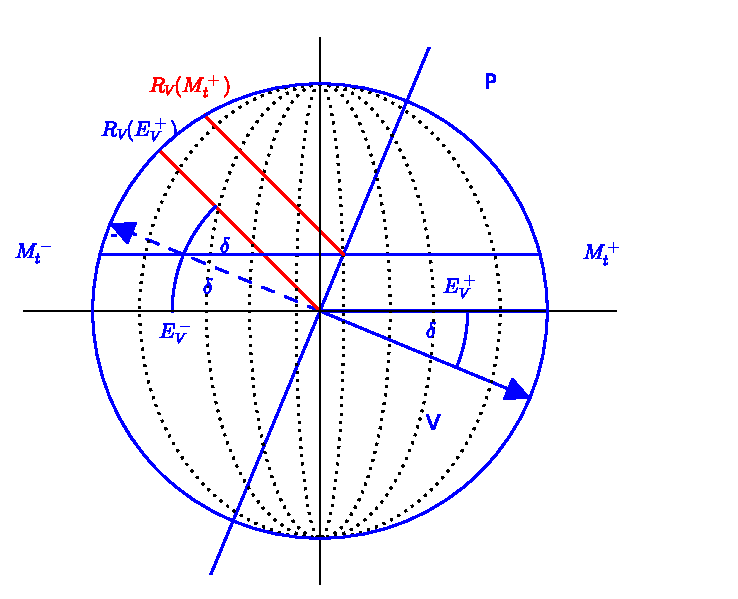
\includegraphics[width=.9\linewidth]{./reflection.pdf}
\caption{Reflection in the $(\vertvec, \reflectionvector)$-plane showing the reflected equator, \(M_T\), \(\reflectionmap(M_t)\) and some geodesics through the north pole (dotted lines).}
\label{fig:reflection}
\end{figure}

This map is an idempotent, (orientation reversing) isometry of \(\R^{n+2}\) fixing \(\reflectionplane\) and in particular fixing the origin. Therefore, it induces an idempotent isometry of \(\S^{n+1}\). Our aim is to show that for any \(\reflectionvector\) with \(\reflectionangle = 0\), the flow \(M_t\) is invariant under \(\reflectionmap\). This will complete the classification since the invariance implies that at each time \(t\), \(M_t\) is contained in a hyperplane orthogonal to \(\vertvec\) and hence must be a geodesic sphere. To achieve this goal, we first work with ``perturbed reflections'' satisying the condition \(\reflectionangle > 0\) to obtain estimates and then finally we send \(\reflectionangle \to 0\). 

The relevant estimates are comparisons of the spherical distance from the reflection \(\reflectionmap(M_t)\) to the equator with the spherical distance of the original hypersurface \(M_t\) to the equator. With this comparison in mind, let \(\radialdistance(x) = d_{\S^{n+1}} (\equator, x) \subseteq [-\pi/2,\pi/2]\) denote the signed, spherical distance from \(\equator\) to \(x \in \S^{n+1}\) with \(H^{\pm} = \{\pm \radialdistance > 0\}\). The radial projection onto \(\equator\) is the map \(x \in \S^{n+1} \mapsto \radialprojection(x) \in \equator\), where \(\radialprojection\) is the nearest point on \(\equator\) to \(x\). If \(x \ne \pm \basepoint\), then \(\radialprojection(x)\) is a single point. If \(x = \pm \basepoint\), then \(\radialprojection(x) = \equator\). In any event, given \(y \in \radialprojection(x)\), there is a unique length minimizing geodesic joining \(x\) to \(y\) and this geodesic must pass through \(\pm \basepoint\). For graphs over the equator \(\{r = f(\sigma) : \sigma \in \equator\}\), each such geodesic intersects the graph in exactly one point.

The height function is \(\height(x) = \ip{x}{\vertvec}\) and is related to the radial distance via
\[
\height(x) = \sin(\radialdistance(x))
\]
which is monotonically increasing in \(\radialdistance\). This monotone relation allows us to work with the height function \(h\) in the ambient Euclidean space \(\R^{n+2}\) rather than the spherical distance \(\radialdistance\) resulting in much simpler calcuations.

For \(x \in \equator\), we have \(\ip{x}{\vertvec} = 0\) and
\begin{equation}
\label{eq:equatorheight}
\height(\reflectionmap(x)) = \ip{\vertvec}{x - 2 \ip{x}{\reflectionvector} \reflectionvector} = 2 \sin\reflectionangle \ip{x}{\reflectionvector}.
\end{equation}
In the case \(x \in \reflectionset{\equator}^+\), we have \(\ip{x}{\reflectionvector} > 0\) and hence \(\height(\reflectionmap(x)) > 0\). In the case \(x \in \equator \intersect \reflectionplane\), we have \(\ip{x}{\reflectionvector} = 0\) and hence \(\height(\reflectionmap(x)) = 0\). This allows us to compare \(\reflectionset{(\reflectionmap(\equator))}^-\) on which \(\height\geq 0\) (equality occuring precisely on the boundary \(\equator \intersect \reflectionplane\)) with \(\reflectionset{\equator}^-\) on which \(\height = 0\). For any hypersurface close to \(\equator\) we will then obtain a similar relation. The major difficulty occurs on the moving boundary \(M_t \intersect \reflectionplane\) on which both sets have \(\height = 0\). To make this comparison precise, we define the following relation:

\begin{definition}
For subsets \(S,T \subset \S^{n+1}\), we say \emph{\(S\) one-sided reflects above \(T\)}, written \(\reflectionmap(S^+) \geq T^-\) provided \(\radialdistance(x) \leq \radialdistance(y)\) for every \(x \in S^+\) and every \(y \in \radialprojection^{-1} (\reflectionmap(x)) \intersect T^-\). Equivalently we may require \(\height(x) \geq \height(y)\).
\end{definition}

In other words, on \(\reflectionhalfspace^-\), the minus side of \(\reflectionplane\), the reflection \(\reflectionmap(S)\) lies ``above'' \(T\).

From now on we assume that \(M_t \subset H^+\), that \(M_t \to \equator\) in \(C^1\) as \(t \to -T_S\) with a uniform \(C^2\) bound, and that \(M_t\) evolves by a parabolic equation, uniform in any region with \(h \geq C g\) for \(C>0\). These assumptions imply we may write \(M_t\) as the graph of a \(C^1\), positive function over \(\equator\) in geodesic polar coordinates: \(M_t = \{r = f_t(\sigma) \in (0,\pi/2) : \sigma \in \equator\)\} for all \(t \in (-T_S, \bar{T}_{\reflectionangle})\) with \(\bar{T}_{\reflectionangle}\) sufficiently close to \(T_S\). Moreover, for \(\reflectionangle \in (0,\pi/4)\), \(\reflectionmap(\equator) = \{r = g_{-T_S}(\sigma)\}\) is a graph over \(\equator\) with \(\ip{\nor_{\reflectionangle}}{\vertvec}\) a constant in \((0,1]\) where \(\nor_{\reflectionangle}\) is the unit normal to \(\reflectionmap(\equator)\) (which is the intersection of a hyperplane and \(\S^{n+1}\)). Since \(\reflectionmap\) is an isometry, \(\reflectionmap(M_t) \to \reflectionmap(\equator)\) in \(C^1\) as \(t \to -T_S\) and hence, increasing \(\bar{T}_{\reflectionangle}\) if necessary, we also have that \(\reflectionmap(M_t) = \{r = g_t(\sigma)\}\) is a graph for all \(t \in (-T_S, \bar{T}_{\reflectionangle})\).

We will make use of monotonicity in \(\reflectionangle\): the constant, \(\ip{\nor_{\reflectionangle}}{\vertvec}\) is monotonically increasing to \(1\) as \(\reflectionangle \to 0\). This just says that \(\nor_{\reflectionangle}\) becomes more vertical as \(\reflectionangle\) decreases and that when \(\reflectionangle = 0\), we have \(\nor_{\reflectionangle} = \vertvec\) (since \(\equator\) is invariant under \(\reflectionmap\)). To give us a little room away from \(\pi/4\) where the reflected equator is no longer a graph, fix any \(\reflectionangle_0 \in (0,\pi/4)\). Letting \(\bar{T} = \bar{T}_{\reflectionangle_0} < T_S\), from the monotonicity in \(\reflectionangle\), both \(M_t\) and \(\reflectionmap(M_t)\) are graphs for all \(t \in (-T_S, -\bar{T})\) and all \(\reflectionangle \in [0,\reflectionangle_0]\).

In the following sequence of lemmas, under the above assumptions, we prove that the hypersurface \(M_t\) one-sided reflects above itself on the interval \((-T_S, -\bar{T})\) for any \(\reflectionangle \in (0, \reflectionangle_0)\).

Let \(C\subset \equator\) be any great circle and consider \(f_t|_C\). The Backwards Approximate Symmetry Lemma \cite[Lemma 5.1]{bryanlouie} applies whenever \(f_t|_C\) converges in \(C^2\) to \(C\) to show that there is a \(T_{\reflectionangle} \in (0, T_S)\) such that
\[
\reflectionmap(\reflectionset{(M_t)}^+) \geq \reflectionset{(M_t)}^-
\]
over any \(C\) and on a neighbourhood of \(\reflectionplane\) in \(\reflectionhalfspace\) for all \(t \in (-T_S, -T_{\reflectionangle})\).

Here we weaken the assumpions to only require \(C^1\) convergence with a uniform \(C^2\) bound. This seems the best we can hope for in general as is remarked in the proof. The proof is similar to the Backwards Approximate Symmetry Lemma, but now we need to obtain better estimates on the neighbourhood. The tricky part is dealing with the moving boundary \(M_t \intersect \reflectionplane\).

\begin{lemma}
\label{lem:approximate_symmetry}
For any \(\reflectionangle \in (0,\reflectionangle_0)\) there exists a \(T_{\reflectionangle} \in (0, T_S)\) such that \((\reflectionset{\reflectionmap(M_t))}^- \geq M_t^-\) for all \(t \in (-T_S, -T_{\reflectionangle})\).
\end{lemma}

\begin{proof}

\emph{Boundary Estmates}

Let \(C\subset \equator\) be any great circle and consider \(f_t|_C\), \(g_t|_C\). We use the Taylor expansions near the two points \(\reflectionplane \intersect M_t = \{x_1(t), x_2(t)\}\) over \(C\). We work near \(x_1(t)\) (the proof being the same near \(x_2\)). For each \(t\), parametrise \(C\) with \(\theta\) such that \(\radialprojection(x_1(t))\) corresponds to \(\theta = 0\) and \(\radialprojection^{-1}\{\theta>0\} \intersect M_t\) lies in \(\reflectionhalfspace^-\). Note that since \(\reflectionmap\) preserves \(\reflectionplane\), we have \(f_t(0) = g_t(0)\) and thus the Taylor expansion with second order remainder is
\[
g_t(\theta) - f_t (\theta) = (g_t'(0) - f_t'(0)) \theta + R \theta^2
\]
where \(R\) is bounded depending only on the uniform bounds for \(f_t''\) (note \(g_t'' = f_t''\)). Since \(M_t \to \equator\) in \(C^1\), as \(t\to -T_S\) we have that \(f_t' \to 0\) and \(g_t' \to \tan(2\reflectionangle)\), the latter being the slope of the reflected equator. Thus there is a \(T_{\reflectionangle}\) such that \(g_t'(0) - f_t'(0)\) is arbitrarily close to the positive constant \(\tan(2\reflectionangle) > 0\) and hence the first order term is positive for all \(t \in (-T_S, T_{\reflectionangle})\). We can easily estimate the interval on which \(g_t(\theta) \geq f_t (\theta)\): The uniform bounds on \(f_t''\) imply that
\[
\eta = \inf_{t \in (-T_S, T_{\reflectionangle})} \frac{g_t'(0) - f_t'(0)}{|R|} > 0
\]
and thus \(g_t(\theta) \geq f_t (\theta)\) on the interval \([0, \eta)\) for any \(t \in (-T_S, T_{\reflectionangle})\). Note that previously in the Backwards Approximate Symmetry Lemma, \(C^2\) convergence to \(0\) implied that \(R\to 0\) and hence by taking \(t\) close enough to \(-T_S\) we could make \(\eta\) arbitrarily large. This of course does not apply with the relaxed assumptions of \(C^2\) bounds only, but it turns out that all we require is \(\eta > 0\). Note also that without uniform \(C^2\) bounds, \(\eta\) may in fact be \(0\) and this is where the final argument below may fail.

Now we can let \(C\) vary and observe that we can make \(g_t'(0) - f_t'(0) > 0\) and \(|R|\) bounded independently of \(C\) by the uniform \(C^1\) convergence and uniform \(C^2\) bound, thus obtaining \(\eta\) independent of \(C\). 

Now, \(\reflectionplane \intersect H^+\) projects onto \(\reflectionset{\equator}^+\), and so \(\radialprojection(x_1(t)) \in \reflectionset{\equator}^+\) and we need to extend our boundary estimate over to \(\reflectionset{\equator}^-\). By decreasing \(T_{\reflectionangle}\) if necessary, as \(M_t\intersect\reflectionplane \to \equator\intersect\reflectionplane\) we have that \(\radialprojection(M_t\intersect\reflectionplane) \subseteq \{x \in \equator : d(x, \reflectionplane) < \eta/2\}\) for all \(t \in (-T_S, T_{\reflectionplane})\). Note that \(\radialprojection(x_1(t))\) is contained is this set, and \(g_t(\theta) \geq f_t (\theta)\) holds for \(\theta\) such \(d(\radialprojection(x_1(t)), C(\theta)) < \eta\) if \(\theta\) is the arc-length parameter of \(C\). This is true for any \(C\), hence holds on \(\{x \in \reflectionset{\equator}^+ : d(x, \reflectionplane) < \eta/2\}\). In geodesic coordinates, for graphs the condition \(\reflectionmap(\reflectionset{(M_t)}^+) \geq \reflectionset{(M_t)}^-\)is equivalent to \(g_t(\theta) \geq f_t (\theta)\) hence we obtain
\begin{equation}
\label{eq:boundaryestimate}
\reflectionmap(\reflectionset{(M_t)}^+) \geq \reflectionset{(M_t)}^- \quad \text{ over } \{x \in \reflectionset{\equator}^+: d(x, \reflectionplane) < \eta/2\}
\end{equation}
and all \(t \in (-T_S, T_{\reflectionangle})\).

\emph{Interior Estmates}

As noted above, \(\height(\reflectionmap(x)) > 0\) on \(\reflectionset{\equator}^+\) and \(\radialdistance = \arcsin(\height(x))\). For any \(\mu > 0\), let
\[
\reflectionset{\equator}^{+,\mu} = \{x \in \reflectionset{\equator}^+: d(x, \equator \intersect \reflectionplane) > \mu\},
\]
and let
\[
G_{\mu} = \inf\{d(\reflectionmap(x), \equator) : x \in \reflectionset{\equator}^{+,\mu}\} > 0.
\]
Since \(M_t \to_{C^0} \equator\), we may choose \(T_{\reflectionangle} \in (0, T_S)\) such that \(d(M_t, \equator) < G_{\reflectionangle}/2\) for all \(t < -T_{\reflectionangle}\); that is, \(\radialdistance (x) < G_{\reflectionangle}/2\) for all \(x \in M_t\) and \(t < -T_{\reflectionangle}\). Now for \(x \in M_t^+ \intersect \radialprojection^{-1} \equator_{\mu}\), since \(\reflectionmap\) is an isometry, we have \(d(\reflectionmap(x), \reflectionmap(\radialprojection(x))) < G_{\reflectionangle}/2\); therefore, \(\radialdistance(\reflectionmap(x)) > G_{\reflectionangle}/2\). Consequently, on \(\reflectionset{\equator}^{+,\mu}\), we have \(\radialdistance(\reflectionmap(\reflectionset{(M_t)}^+)) > G_{\reflectionangle}/2\) and \(\radialdistance(M_t^-) > G_{\reflectionangle}/2\). In other words, given any \(\mu>0\), there is a \(T_{\reflectionangle}\) such that for all \(t \in (-T_S,T_{\reflectionangle})\),  we have
\begin{equation}
\label{eq:interiorestimate}
\reflectionmap(\reflectionset{(M_t)}^+) \geq \reflectionset{(M_t)}^- \quad \text{ over } \reflectionset{\equator}^{+,\mu}.
\end{equation}

\emph{Combined Estmates}

Choose \(T_{\reflectionangle}\) and \(\eta\) so that both the boundary estimate \cref{eq:boundaryestimate} holds. Now choose \(\mu\) so that \(\radialprojection(\reflectionmap(\reflectionset{\equator}^{+,\mu})) \union \{x \in \reflectionset{\equator}^- : d(x, \reflectionplane) = \reflectionset{\equator}^-\) which can be achieved since \(\reflectionmap\) is an isometry. Decreasing \(T_{\delta}\) if necessary ensures that the interior estimate \cref{eq:interiorestimate} also holds and hence,
\[
\reflectionmap(\reflectionset{(M_t)}^+) \geq \reflectionset{(M_t)}^-
\]
everywhere for all \(t \in (-T_S, -T_{\reflectionangle})\).
\end{proof}

\begin{lemma}
\label{lem:approximate_symmetrypreserved}
There exists a \(T\) independent of \(\reflectionangle\) such that for any \(\reflectionangle \in (0,\reflectionangle_0)\) we have \(\reflectionmap(\reflectionset{M_t^+}) \geq M_t^-\) for all \(t \in (-T_S, -T)\).
\end{lemma}

\begin{proof}
As remarked above, there exists a \(T\) such that both \(M_t\) and \(\reflectionmap(M_t\) are graphs over the equator on \((-T_S, T)\). Moreover, since both the equator \(\equator\) and the reflected equator \(\reflectionmap(\equator)\) meet \(\reflectionplane\) transversely, be decreasing \(T\) if necessary, we may assume \(M_t\) and \(\reflectionmap(M_t\) also meet \(\reflectionplane\) transversely. As with the monotonicity of the graph property in \(\reflectionangle\) we have monotonicity in transerval meeting and so \(T\) is independent of \(\reflectionangle\)..

Recall the assumption that \(M_t\) satsifies a uniformly parabolic equation wherever it is strictly convex. Since \(\reflectionmap\) is an isometry, \(\reflectionmap(M_t)\) also is strictly convex and satisfies the same equation. Therefore \(f_t,g_t\) satisfy a uniformly parabolic equation on \((-T_S + \epsilon_{\reflectionangle}, -T)\) where \(0 < epsilon_{\reflectionangle} < \min\{T_S-T, T_S-T_{\reflectionangle}\}\) is chosen so that we have a strict, positive lower bound on \(|A|\) from strict convexity and compactness and so that on \((-T_S + \epsilon_{\reflectionangle}, -T_{\reflectionangle})\) we have the condition \(\reflectionmap(\reflectionset{(M_t)}^+) \geq \reflectionset{(M_t)}^-\). That is, \(g_t \geq f_t\). We also have the boundary condition \(f_t = g_t\) on \(\reflectionplane\).

Now we may apply the maximum principle on the parabolic domain \(\union_{t \in (-T_S + \epsilon_{\reflectionangle}, -T)} \radialprojection(\reflectionset(M_t)^-) \subseteq \equator\) to conclude that \(g_t \geq f_t\) holds forwards in time on all of \((-T_S + \epsilon_{\reflectionangle}, -T)\) hence on all of \((-T_S, -T)\). Note that we use the maximum principle almost verbatim as stated in \cite[3.7, Theorem 12]{MR762825} except that this theorem is stated only for cylindrical domains \(\Omega \times (-T_S + \epsilon, -T)\) whereas our domain has a changing boundary. Nevertheless, a closer look at the proof reveals that it only relies on the maximum princple for the linearised equation \cite[3.3, Theorem 7, remark (ii)]{MR762825} which does hold on time dependent domains. Alternatively, one can rule out \(f_t\) touching \(g_t\) near the boundary by the parabolic Hopf boundary point lemma \cite[3.3, Theorem 6]{MR762825} (which holds for our domains since they satisfy the interior sphere condition and is only needed for the linearisation) and then rule out interior touching by the usual contradiction argument such as in \cite[3.2 Lemma]{MR837523}.
\end{proof}

\begin{theorem}
\label{thm:classification}
Let \(M_t\) be a convex, embedded (quasi-)ancient solution of any (uniform whenever on uniformly convex hypersurfaces) parabolic equation on \(\S^{n+1}\) such that \(M_t \to \equator\) in \(C^1\) as \(t \to -T_S\) with uniform \(C^2\) bounds. Then \(M_t\) is a family of shrinking geodesic spheres emanating from the equator \(\equator\) at \(t=-T_S\).
\end{theorem}

\begin{proof}
From \cref{lem:approximate_symmetrypreserved} we have \(\reflectionmap(\reflectionset{(M_t)}^+) \geq \reflectionset{(M_t)}^-\) everywhere for all \(t \in (-T_S, -T)\) and any \(\reflectionangle \in (0,\reflectionangle_0)\). By continuity therefore, sending \(\reflectionangle \to 0\) we have \(\reflectionmap(\reflectionset{(M_t)}^+) \geq \reflectionset{(M_t)}^-\) for all \(t \in (-T_S, -T)\)  and any \(\reflectionvector\) satisfying \(\ip{\reflectionvector}{\vertvec} = 0\).

Now, we need some simple properties of $\reflectionmap[\reflectionvector_0]$ following from the fact that $\ip{\reflectionvector}{\vertvec} = 0$:
\begin{itemize}
\item $\reflectionmap^2 = \id$,
\item $S \geq T \Rightarrow \reflectionmap(S) \geq  \reflectionmap(T)$,
\item $\reflectionmap = \reflectionmap[-\reflectionvector]$, and
\item $\reflectionset{S}^{\pm} = \reflectionset[-\reflectionvector]{S}^{\mp}$.
\end{itemize}

Thus we obtain,
\begin{align*}
\reflectionset{(M_t)}^+ &= \reflectionmap(\reflectionmap(\reflectionset{(M_t)}^+)) \geq \reflectionmap(\reflectionset{(M_t)}^-) \\
&= \reflectionmap[-\reflectionvector](\reflectionset[-\reflectionvector]{(M_t)^+}) \geq \reflectionset[-\reflectionvector]{(M_t)}^-\\
&= \reflectionset{(M_t)}^+.
\end{align*}
We must have equality all the way through and hence the middle line implies
\[
\reflectionmap[-\reflectionvector](\reflectionset[-\reflectionvector]{(M_t)^+}) = \reflectionset[-\reflectionvector]{(M_t)}^-
\]
for any $\reflectionvector$.

Thus \(M_t\) is invariant under \(\reflectionmap\) for any \(\reflectionvector\) satisfying \(\ip{\reflectionvector}{\vertvec} = 0\) and hence is a geodesic sphere for every \(t \in (-T_S, T)\) and by uniqueness of solutions, is a geodesic sphere for every \(t \in (-T_S, 0)\).
\end{proof}


\bibliographystyle{amsplain}
\bibliography{Bibliography.bib}


\end{document}
